\documentclass[journal,12pt,twocolumn]{IEEEtran}

\usepackage{setspace}
\usepackage{gensymb}
\singlespacing
\usepackage[cmex10]{amsmath}
\usepackage{cancel}
\usepackage{amsthm}

\usepackage{paralist}

\usepackage{mathrsfs}
\usepackage{txfonts}
\usepackage{stfloats}
\usepackage{bm}
\usepackage{cite}
\usepackage{cases}
\usepackage{subfig}

\usepackage{longtable}
\usepackage{multirow}
\usepackage{enumitem}
\usepackage{mathtools}
\usepackage{steinmetz}
\usepackage{tikz}
\usepackage{circuitikz}
\usepackage{verbatim}
\usepackage{tfrupee}
\usepackage[breaklinks=true]{hyperref}
\usepackage{graphicx}
\usepackage{tkz-euclide}

\usetikzlibrary{calc,math}
\usepackage{listings}
    \usepackage{color}                                            %%
    \usepackage{array}                                            %%
    \usepackage{longtable}                                        %%
    \usepackage{calc}                                             %%
    \usepackage{multirow}                                         %%
    \usepackage{hhline}                                           %%
    \usepackage{ifthen}                                           %%
    \usepackage{lscape}     
\usepackage{multicol}
\usepackage{chngcntr}

\DeclareMathOperator*{\Res}{Res}
\usepackage{romannum}
\renewcommand\thesection{\arabic{section}}
\renewcommand\thesubsection{\thesection.\arabic{subsection}}
\renewcommand\thesubsubsection{\thesubsection.\arabic{subsubsection}}

\renewcommand\thesectiondis{\arabic{section}}
\renewcommand\thesubsectiondis{\thesectiondis.\arabic{subsection}}
\renewcommand\thesubsubsectiondis{\thesubsectiondis.\arabic{sub subsection}}


\hyphenation{optical networks semiconduc-tor}
\def\inputGnumericTable{}                                 %%

\lstset{
%language=C,
frame=single, 
breaklines=true,
columns=fullflexible
}
\date{March 2021}

\begin{document}
\theoremstyle{definition}
\newtheorem{definition}{Definition}[section]

\newcommand{\BEQA}{\begin{eqnarray}}
\newcommand{\EEQA}{\end{eqnarray}}
\newcommand{\define}{\stackrel{\triangle}{=}}
\bibliographystyle{IEEEtran}
\raggedbottom
\setlength{\parindent}{0pt}
\providecommand{\mbf}{\mathbf}
\providecommand{\pr}[1]{\ensuremath{\Pr\left(#1\right)}}
\providecommand{\qfunc}[1]{\ensuremath{Q\left(#1\right)}}
\providecommand{\fn}[1]{\ensuremath{f\left(#1\right)}}
\providecommand{\e}[1]{\ensuremath{E\left(#1\right)}}
\providecommand{\sbrak}[1]{\ensuremath{{}\left[#1\right]}}
\providecommand{\lsbrak}[1]{\ensuremath{{}\left[#1\right.}}
\providecommand{\rsbrak}[1]{\ensuremath{{}\left.#1\right]}}
\providecommand{\brak}[1]{\ensuremath{\left(#1\right)}}
\providecommand{\lbrak}[1]{\ensuremath{\left(#1\right.}}
\providecommand{\rbrak}[1]{\ensuremath{\left.#1\right)}}
\providecommand{\cbrak}[1]{\ensuremath{\left\{#1\right\}}}
\providecommand{\lcbrak}[1]{\ensuremath{\left\{#1\right.}}
\providecommand{\rcbrak}[1]{\ensuremath{\left.#1\right\}}}
\theoremstyle{remark}
\newtheorem{rem}{Remark}
\newcommand{\sgn}{\mathop{\mathrm{sgn}}}
\providecommand{\abs}[1]{\vert#1\vert}
\providecommand{\res}[1]{\Res\displaylimits_{#1}} 
\providecommand{\norm}[1]{\lVert#1\rVert}
%\providecommand{\norm}[1]{\lVert#1\rVert}
\providecommand{\mtx}[1]{\mathbf{#1}}
\providecommand{\mean}[1]{E[ #1 ]}
\providecommand{\fourier}{\overset{\mathcal{F}}{ \rightleftharpoons}}
%\providecommand{\hilbert}{\overset{\mathcal{H}}{ \rightleftharpoons}}
\providecommand{\system}{\overset{\mathcal{H}}{ \longleftrightarrow}}
	%\newcommand{\solution}[2]{\textbf{Solution:}{#1}}
\newcommand{\solution}{\noindent \textbf{Solution: }}
\newcommand{\cosec}{\,\text{cosec}\,}
\providecommand{\dec}[2]{\ensuremath{\overset{#1}{\underset{#2}{\gtrless}}}}
\newcommand{\myvec}[1]{\ensuremath{\begin{pmatrix}#1\end{pmatrix}}}
\newcommand{\mydet}[1]{\ensuremath{\begin{vmatrix}#1\end{vmatrix}}}
\numberwithin{equation}{subsection}
\makeatletter
\vspace{3cm}
\title{Assignment 6}
\author{G SAVARANA DATTA REDDY - AI20BTECH11008}
\maketitle
\newpage
\bigskip
\renewcommand{\thetable}{\theenumi}
Download the python code from 
\begin{lstlisting}
https://github.com/SavaranaDatta/AI1103/tree/main/Assignment_6.py
\end{lstlisting}
%
and latex-tikz code from 
%
\begin{lstlisting}
https://github.com/SavaranaDatta/AI1103/tree/main/Assignment_6.tex
\end{lstlisting}
\section{PROBLEM}
Let X$_{1}$ and X$_{2}$ be a random sample of size two
from a distribution with probability density
function
\begin{align}
    f_{\theta}(x) &= \theta \brak{\dfrac{1}{\sqrt{2\pi}}}e^{-\dfrac{1}{2} x^{2}} + \brak{1-\theta}\brak{\dfrac{1}{2}}e^{-\mid x\mid} \nonumber,
\end{align}
$-\infty<x<\infty$,\\
where  $\theta \in \cbrak{ 0,\dfrac{1}{2}, 1 }$. If the observed values
of X$_{1}$ and X$_{2}$ are 0 and 2, respectively, then
the maximum likelihood estimate of $\theta$ is
\begin{enumerate}
    \item 0 
    \item $\frac{1}{2}$
    \item 1
    \item not unique
\end{enumerate}
\section{SOLUTION}
\begin{definition}[Maximum Likelihood Estimation (MLE)]
In statistics maximum likelihood estimation is a method of estimating the parameters of a probability distribution by maximising a likelihood function so that under the assumed statistical model the observed data is more probable .The point in the parameter space that maximises the likelihood function is called maximum likelihood estimate .
\end{definition}

The likelihood function is given by 
\begin{align}
    L(\theta \hspace{0.1cm}|\hspace{0.1cm}X_{1}=0,X_{2}=2)  &=f_{\theta}(X_{1}=0)\times f_{\theta}(X_{2}=2)\\
    &=\brak{\theta\brak{\dfrac{1}{\sqrt{2\pi}}-\frac{1}{2}}+\frac{1}{2}}^{2}e^{-2} 
\end{align}
\begin{figure}
    \centering
    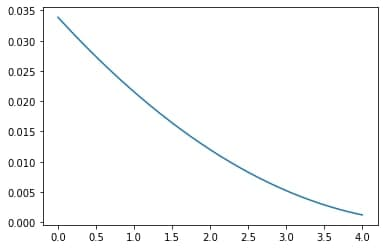
\includegraphics[width=\columnwidth]{Image.jpg}
    \caption{Graph of $L(\theta)$}
\end{figure}
But $\theta \in \cbrak{ 0,\dfrac{1}{2}, 1 }$.
From figure we can see that maximum value of $L(\theta)$ occurs at $\theta=0$.
Therefore required option is \textbf{1}.
\end{document}